\documentclass[a4paper, 12pt]{article}
\usepackage[T2A,T1]{fontenc}
\usepackage[utf8]{inputenc}
\usepackage[english, russian]{babel}
\usepackage{graphicx}
\usepackage[hcentering, bindingoffset = 10mm, right = 15 mm, left = 15 mm, top=20mm, bottom = 20 mm]{geometry}
\usepackage{multirow}
\usepackage{lipsum}
\usepackage{amsmath, amstext}
\usepackage{siunitx}
\usepackage{subcaption}
\usepackage{wrapfig}
\usepackage{mathrsfs}
\usepackage{adjustbox}
\usepackage{enumerate, indentfirst, float}
\usepackage{capt-of, svg}
\usepackage{icomma}
\usepackage{xcolor}
\usepackage{ctable}
\newenvironment{bottompar}{\par\vspace*{\fill}}{\clearpage}
 

\begin{document}
\begin{titlepage}

\newcommand{\HRule}{\rule{\linewidth}{0.5mm}} % Defines a new command for the horizontal lines, change thickness here

\center % Center everything on the page
 
%----------------------------------------------------------------------------------------
%	HEADING SECTIONS
%----------------------------------------------------------------------------------------

\textsc{\LARGE Московский физико-технический институт}\\[1,5cm] % Name of your university/college
\textsc{\Large Кафедра общей физики}\\[0.5cm] % Major heading such as course name
\textsc{\large Лабораторная работа \textnumero  4.3.2}\\[0.5cm] % Minor heading such as course title

%----------------------------------------------------------------------------------------
%	TITLE SECTION
%----------------------------------------------------------------------------------------

\HRule
\\[0.4cm]
{ \huge \bfseries Дифракция света на ультразвуковой волне в жидкости}
\\[0.2cm] % Title of your document
\HRule
\\[1.5cm]


 
%----------------------------------------------------------------------------------------
%	AUTHOR SECTION
%----------------------------------------------------------------------------------------

\begin{minipage}{0.4\textwidth}
	\begin{flushleft} \large
		\emph{Студенты:}\\
		Алексей \textsc{Домрачев} \\
		Нусратилло \textsc{Носиров}\\
		615 группа\\
		
	\end{flushleft}
\end{minipage}
~
\begin{minipage}{0.4\textwidth}
	\begin{flushright} \large
		\emph{Преподаватель:} \\
		Андрей Андреевич \\ \textsc{Заболотных} % Supervisor's Name
	\end{flushright}
\end{minipage}

\begin{bottompar}
	\begin{center}
		
\includegraphics[width = 80 mm]{logo.jpg}
	\end{center}
	{\large \today}

\end{bottompar}
\vfill % Fill the rest of the page with whitespace

\end{titlepage}

\section{Подготовка}
\textbf{Цель работы:} изучение дифракции света на синусоидальной акустической решетке и наблюдение фазовой решетки методом темного поля.
%\vspace{10}\\

\textbf{В работе используются:} оптическая скамья, осветитель, два длиннофокусных объектива, кювета с жидкостью,кварцевый излучатель с микрометрическим винтом,генератор ультразвуковой частоты, линза, вертикальная нить на рейтере, микроскоп.

\subsection*{Экспериментальная установка}

\begin {figure}[H]
	\begin{center}
		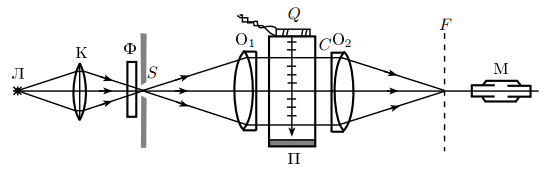
\includegraphics[width = 0.6 \textwidth]{sgBB2_croper_ru.png}
		\caption{Схема наблюдения дифракции на акустической решетке}
	\end{center}
\end {figure}

\begin {figure}[H]
	\begin{center}
		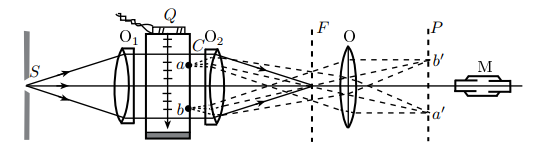
\includegraphics[width = 0.6 \textwidth]{ghmDF_croper_ru.png}
		\caption{Наблюдение акустической решетки методом темного поля}
	\end{center}
\end {figure}

\paragraph{Задание}
В работе предлагается: 
\begin {enumerate}
\item Измерить координаты дифракционных полос, образующихся при дифракции света на акустической решетке.
\item Определить период этой решетки методом темного поля.
\item Рассчитать скорость ультразвука в воде.
\end {enumerate}

\newpage


\section{Работа и измерения}

\subsection*{Установка с вертикальной щелью}
\subsection*{Определение скорости ультразвука по дифракционной картине}

\begin {enumerate}
\item Соберем схему согласно рис.1, подготовим приборы к работе.
\item Заметили, что при увеличении УЗ частоты дифракционная картина размывается и число дифракционных полос уменьшается.
\item С помощью микрометрического винта измерим расстояние между двумя соседними наиболее четкими дифракционным картинами. Оно равно половине длины УЗ волны $ \Lambda/2 = 1.41 \cdot 10^{-3} $ м. Измерения проводились при частоте 1.04 Мгц. Рассчитаем скорость УЗ волны:
\[
	v = \Lambda \nu = 1466\text{ м/с}
\]
\item Измерим положения дифракционных максимумов при той же частоте генератора и частоте равной 2.87МГц и занесем в таблицу \ref{task1}.
\begin{table}[H]
	\centering
	\caption{Положение дифракционных максимумов}
	\label{task1}
	\begin{tabular}{ccc}
		& \multicolumn{2}{c}{Частота} \\ \toprule
		\multicolumn{1}{c|}{} & \multicolumn{1}{c|}{1.04 МГц} & 2.87МГц \\ \midrule
		\multicolumn{1}{c|}{$x_1$, мм} & \multicolumn{1}{c|}{-0.80} & 0.40 \\ \midrule
		\multicolumn{1}{c|}{$x_2$, мм} & \multicolumn{1}{c|}{-0.63} & 0.28 \\ \midrule
		\multicolumn{1}{c|}{$x_3$, мм} & \multicolumn{1}{c|}{-0.54} & 0.02 \\ \midrule
		\multicolumn{1}{c|}{$x_4$, мм} & \multicolumn{1}{c|}{-0.41} & -0.42 \\ \midrule
		\multicolumn{1}{c|}{$x_5$, мм} & \multicolumn{1}{c|}{-0.26} & -0.80 \\ \midrule 
		\multicolumn{1}{c|}{$x_6$, мм} & \multicolumn{1}{c|}{-0.10} & -1.20 \\ \bottomrule
	\end{tabular}
\end{table}
\item Построим по полученным данным следующие графики:

	\begin {figure}[H]
		\begin{center}
			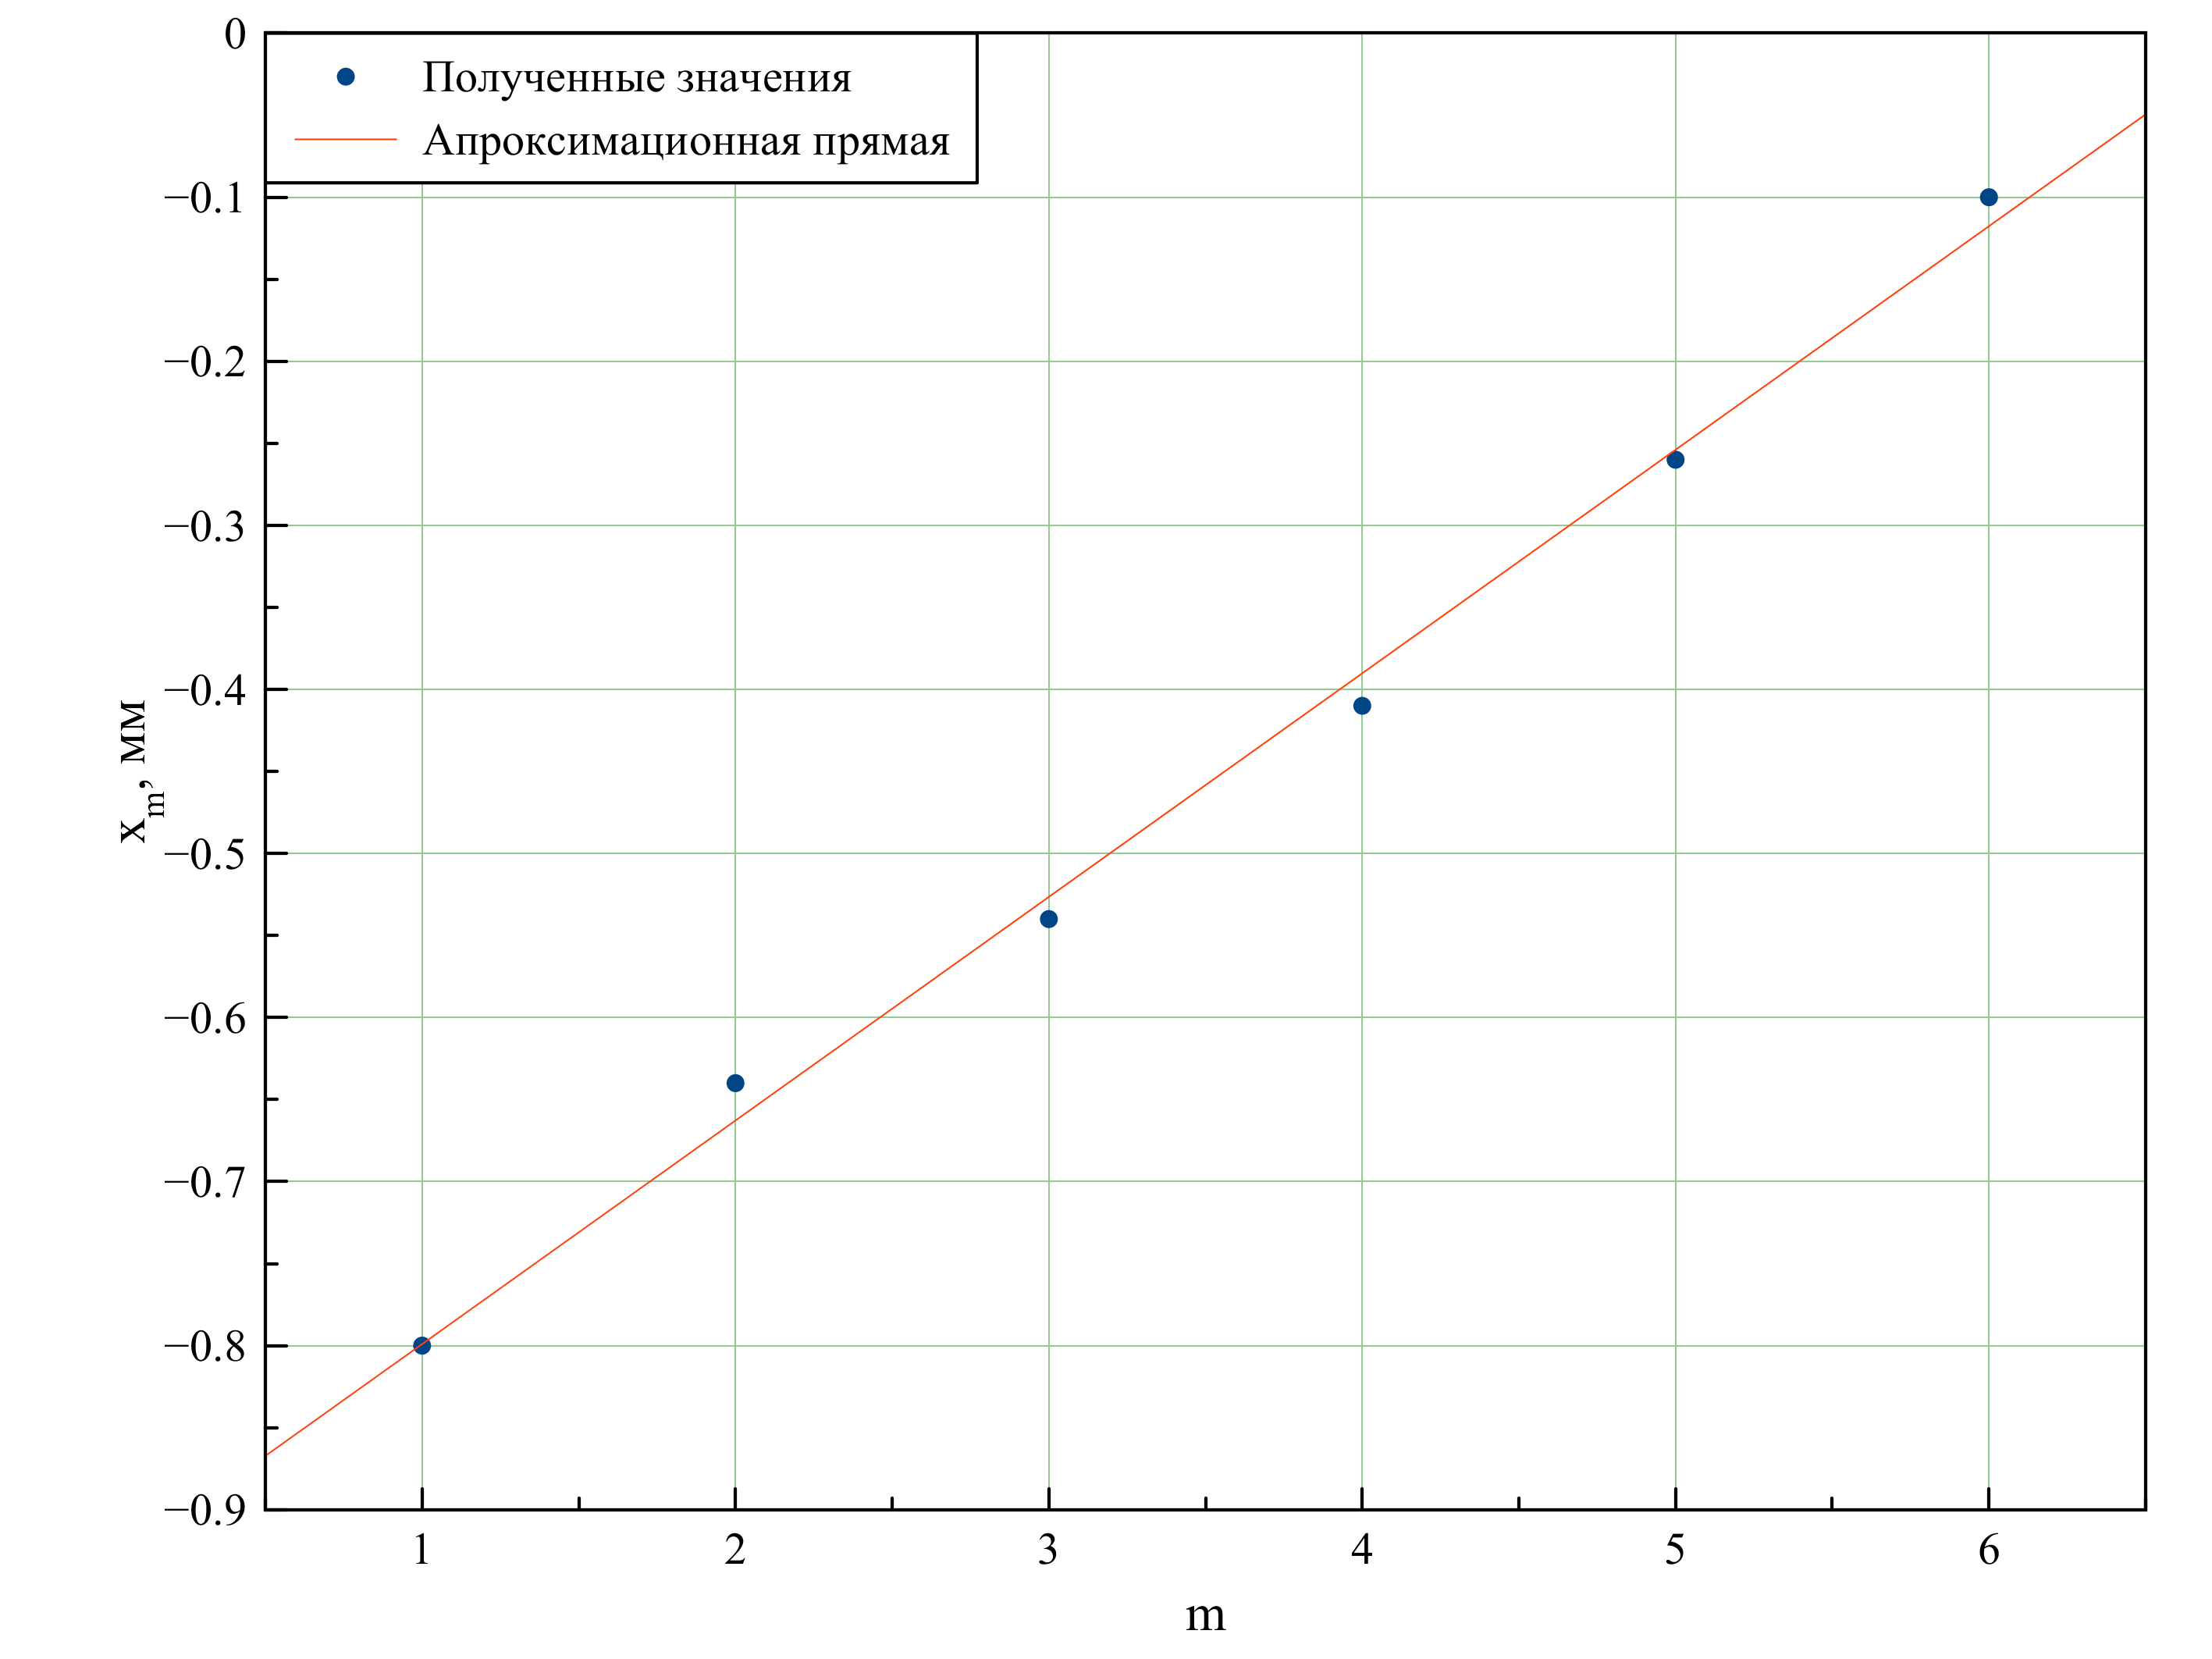
\includegraphics[width = 0.5 \textwidth]{graph1.png}
			\caption{График зависимости координаты дифракционного максимума $x_m$ от порядка m при частоте 1.04 МГц}
		\end{center}
	\end {figure}
	
	\begin {figure}[H]
	\begin{center}
		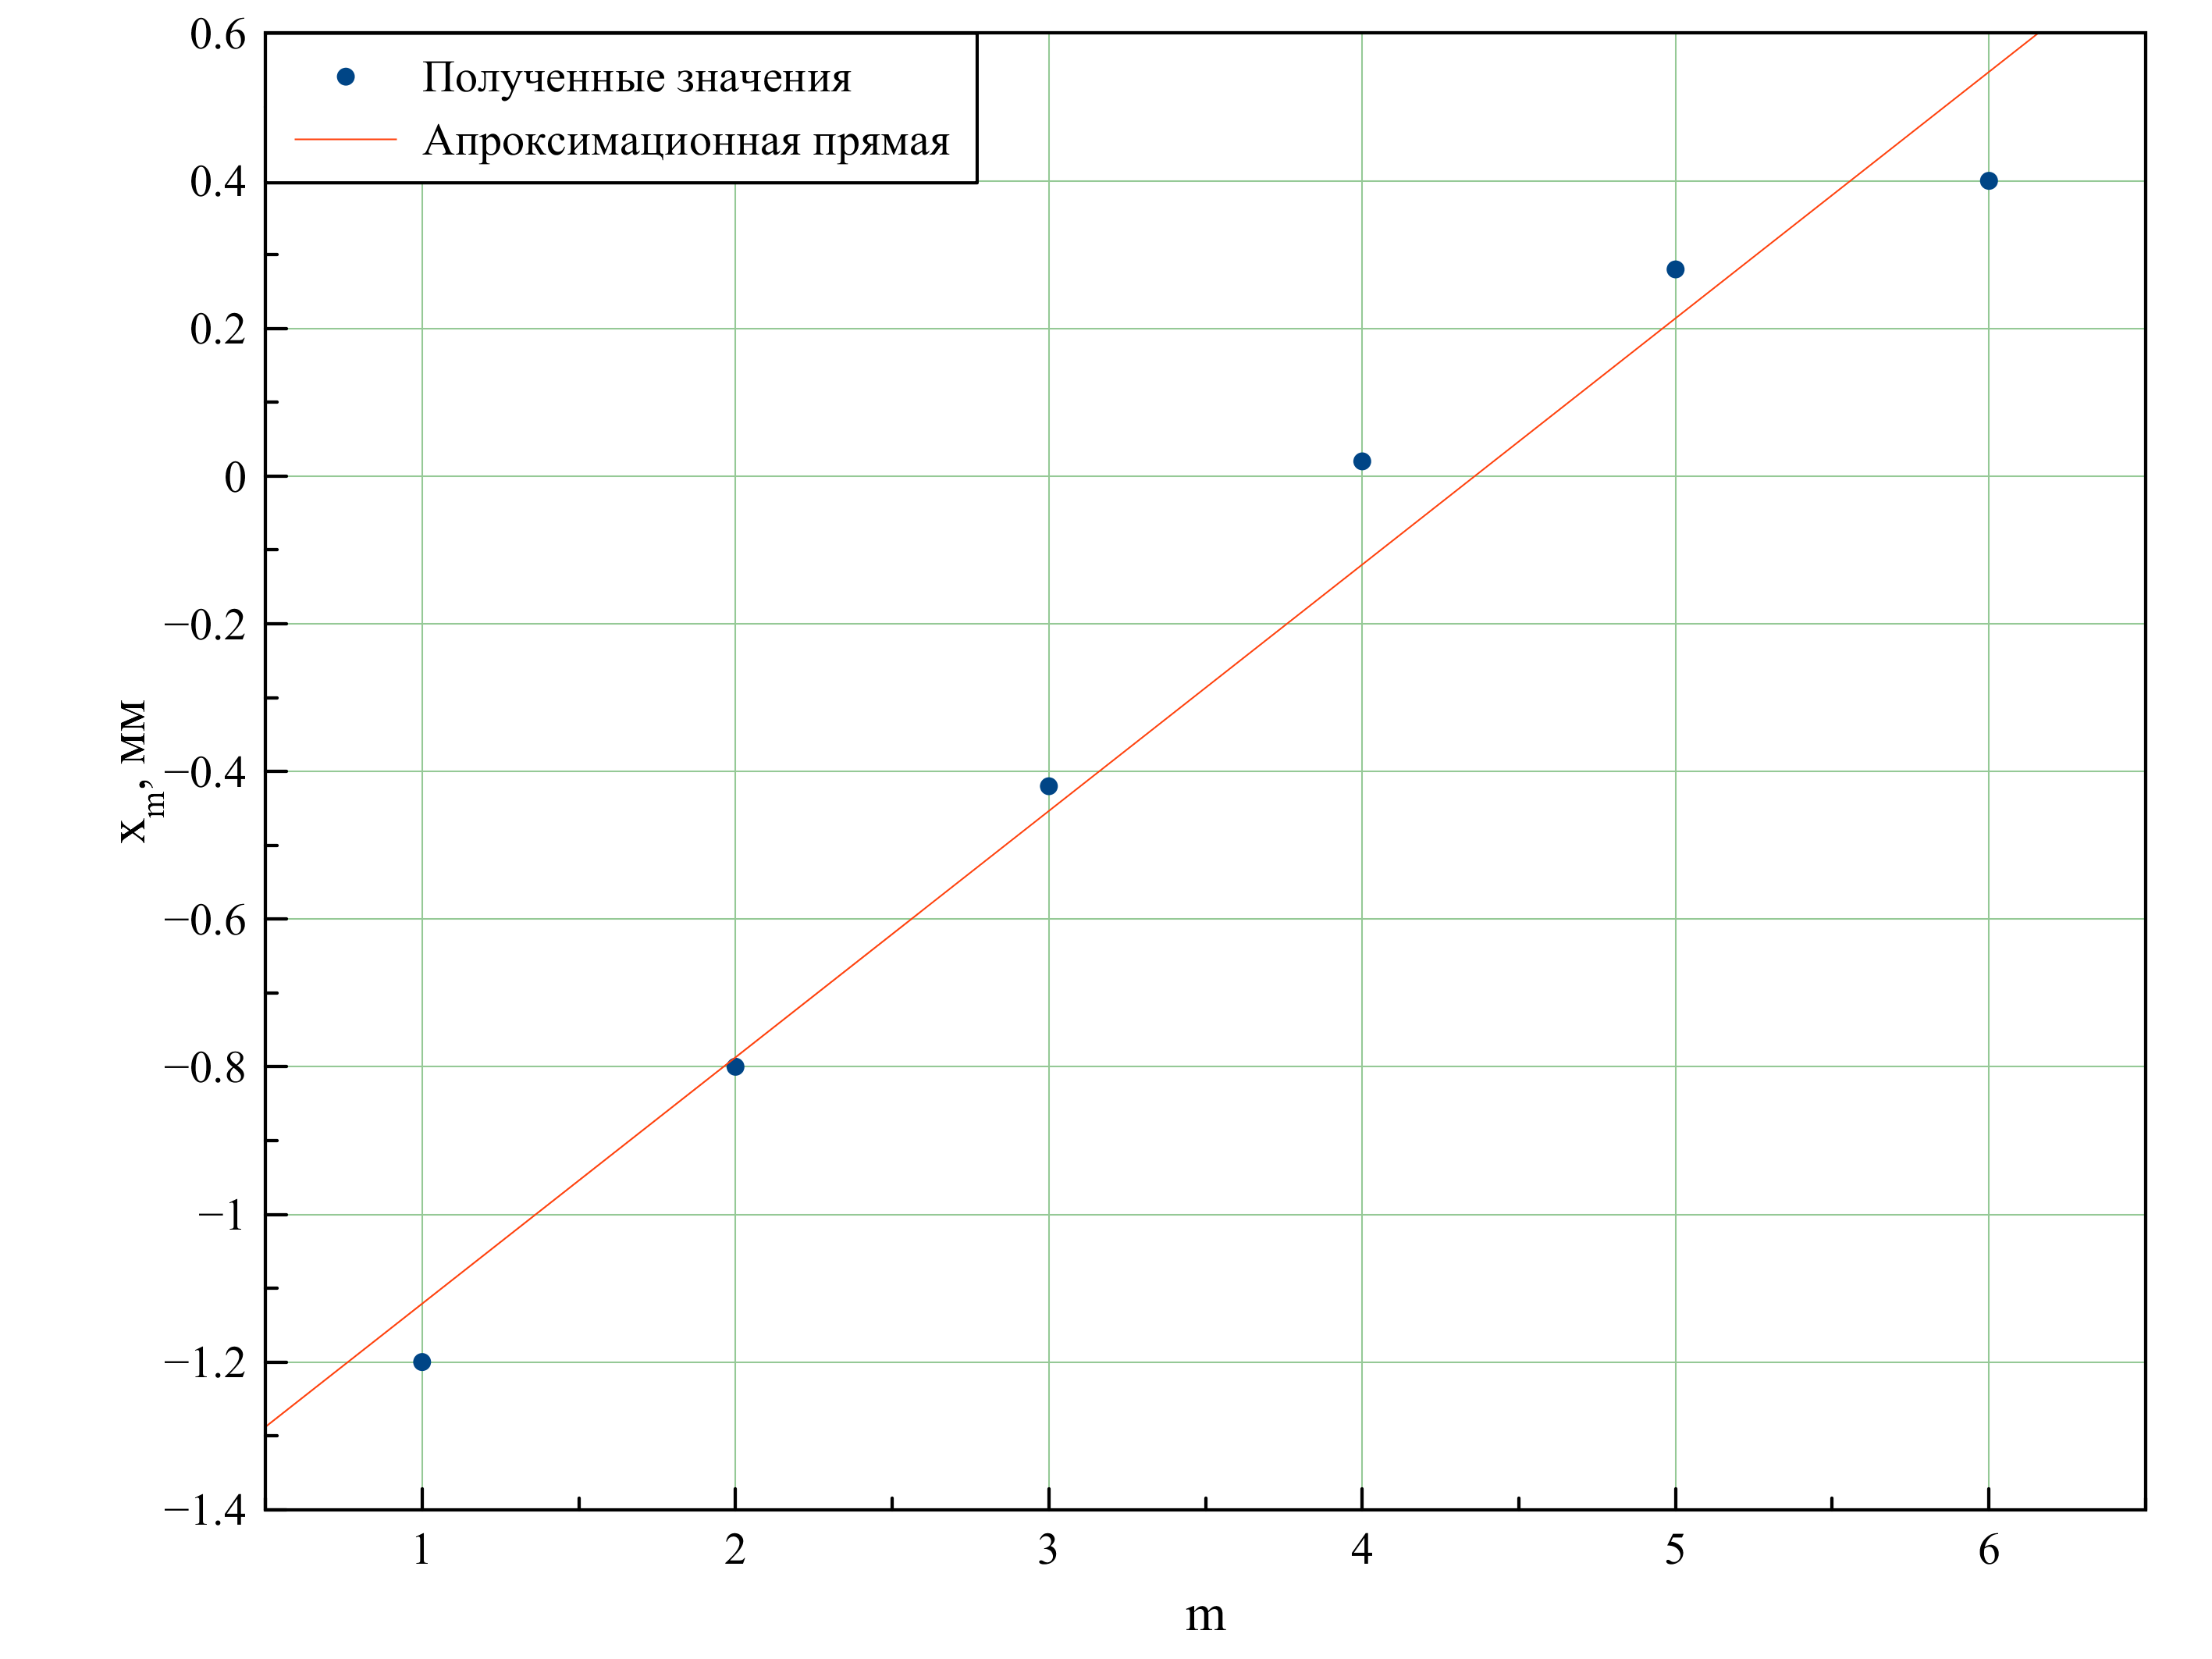
\includegraphics[width = 0.5 \textwidth]{graph2.png}
		\caption{График зависимости координаты дифракционного максимума $x_m$ от порядка m при частоте 2.87 МГц}
	\end{center}
	\end {figure}
	
\item По наклону прямой определим расстояние между соседними полосами: $$l_m/m=\Delta x_m/\Delta m$$
\item Рассчитаем длину УЗ-волны и скорость ультразвука в воде по формулам:
$$\Lambda=f\frac{\lambda}{l_m/m},\ \ \upsilon = \Lambda \nu$$

\begin{table}[H]
\centering
\caption{Результаты}
\label{my-label}
\begin{tabular}{c|c|c|c}

$\nu$, МГц & $ l_m/m$, мм  & $\Lambda,\text{ мм}$ & $\upsilon,\text{ м/с}$ \\ \toprule
1.04    & $ 0.13 \pm 0.01 $ & 1.50 $ \pm $ 0.02     & 1515 $ \pm $ 11           \\ \midrule
2.87    & $ 0.34 \pm 0.01 $ & 0.57 $ \pm $ 0.03     & 1646 $ \pm $ 9           \\ \bottomrule
\end{tabular}
\end{table}
	$$<\upsilon> = 1581 \pm 7\ \text{м/с}$$
\end {enumerate}

\subsection*{Определение скорости ультразвука методом темного поля}
\begin {enumerate}
\item Соберем схему согласно рис.2
\item Проведем калибровку
\item Измерим расстояние между самыми дальними из хорошо видимых в поле зрения темных полос.

\begin{table}[H]
	\centering
	\caption{Метод темного поля}
	\label{dark_pole}
	\begin{tabular}{c|c|c|c|c|c|c}
		
		$\nu,$ МГц & $x_1,\text{ дел}$ & $x_n,\text{ дел}$ & $\Delta x,\text{ дел}$ & $L,\text{ мм}$ & $N,\text{ шт}$ & $\Lambda,\text{ мм}$ \\ \toprule
		1.086     & 7                & 167              & 160                   & 6.40           & 10            & 1.28                \\ \midrule
		1.591     & 0                & 175              & 175                   & 7.00             & 16            & 0.88               \\ \midrule
		1.963     & 5                & 173              & 168                   & 6.72          & 19            & 0.71               \\ \bottomrule
	\end{tabular}
\end{table}
\item Построим по полученным данным следующий график:

    \begin {figure}[H]
		\begin{center}
			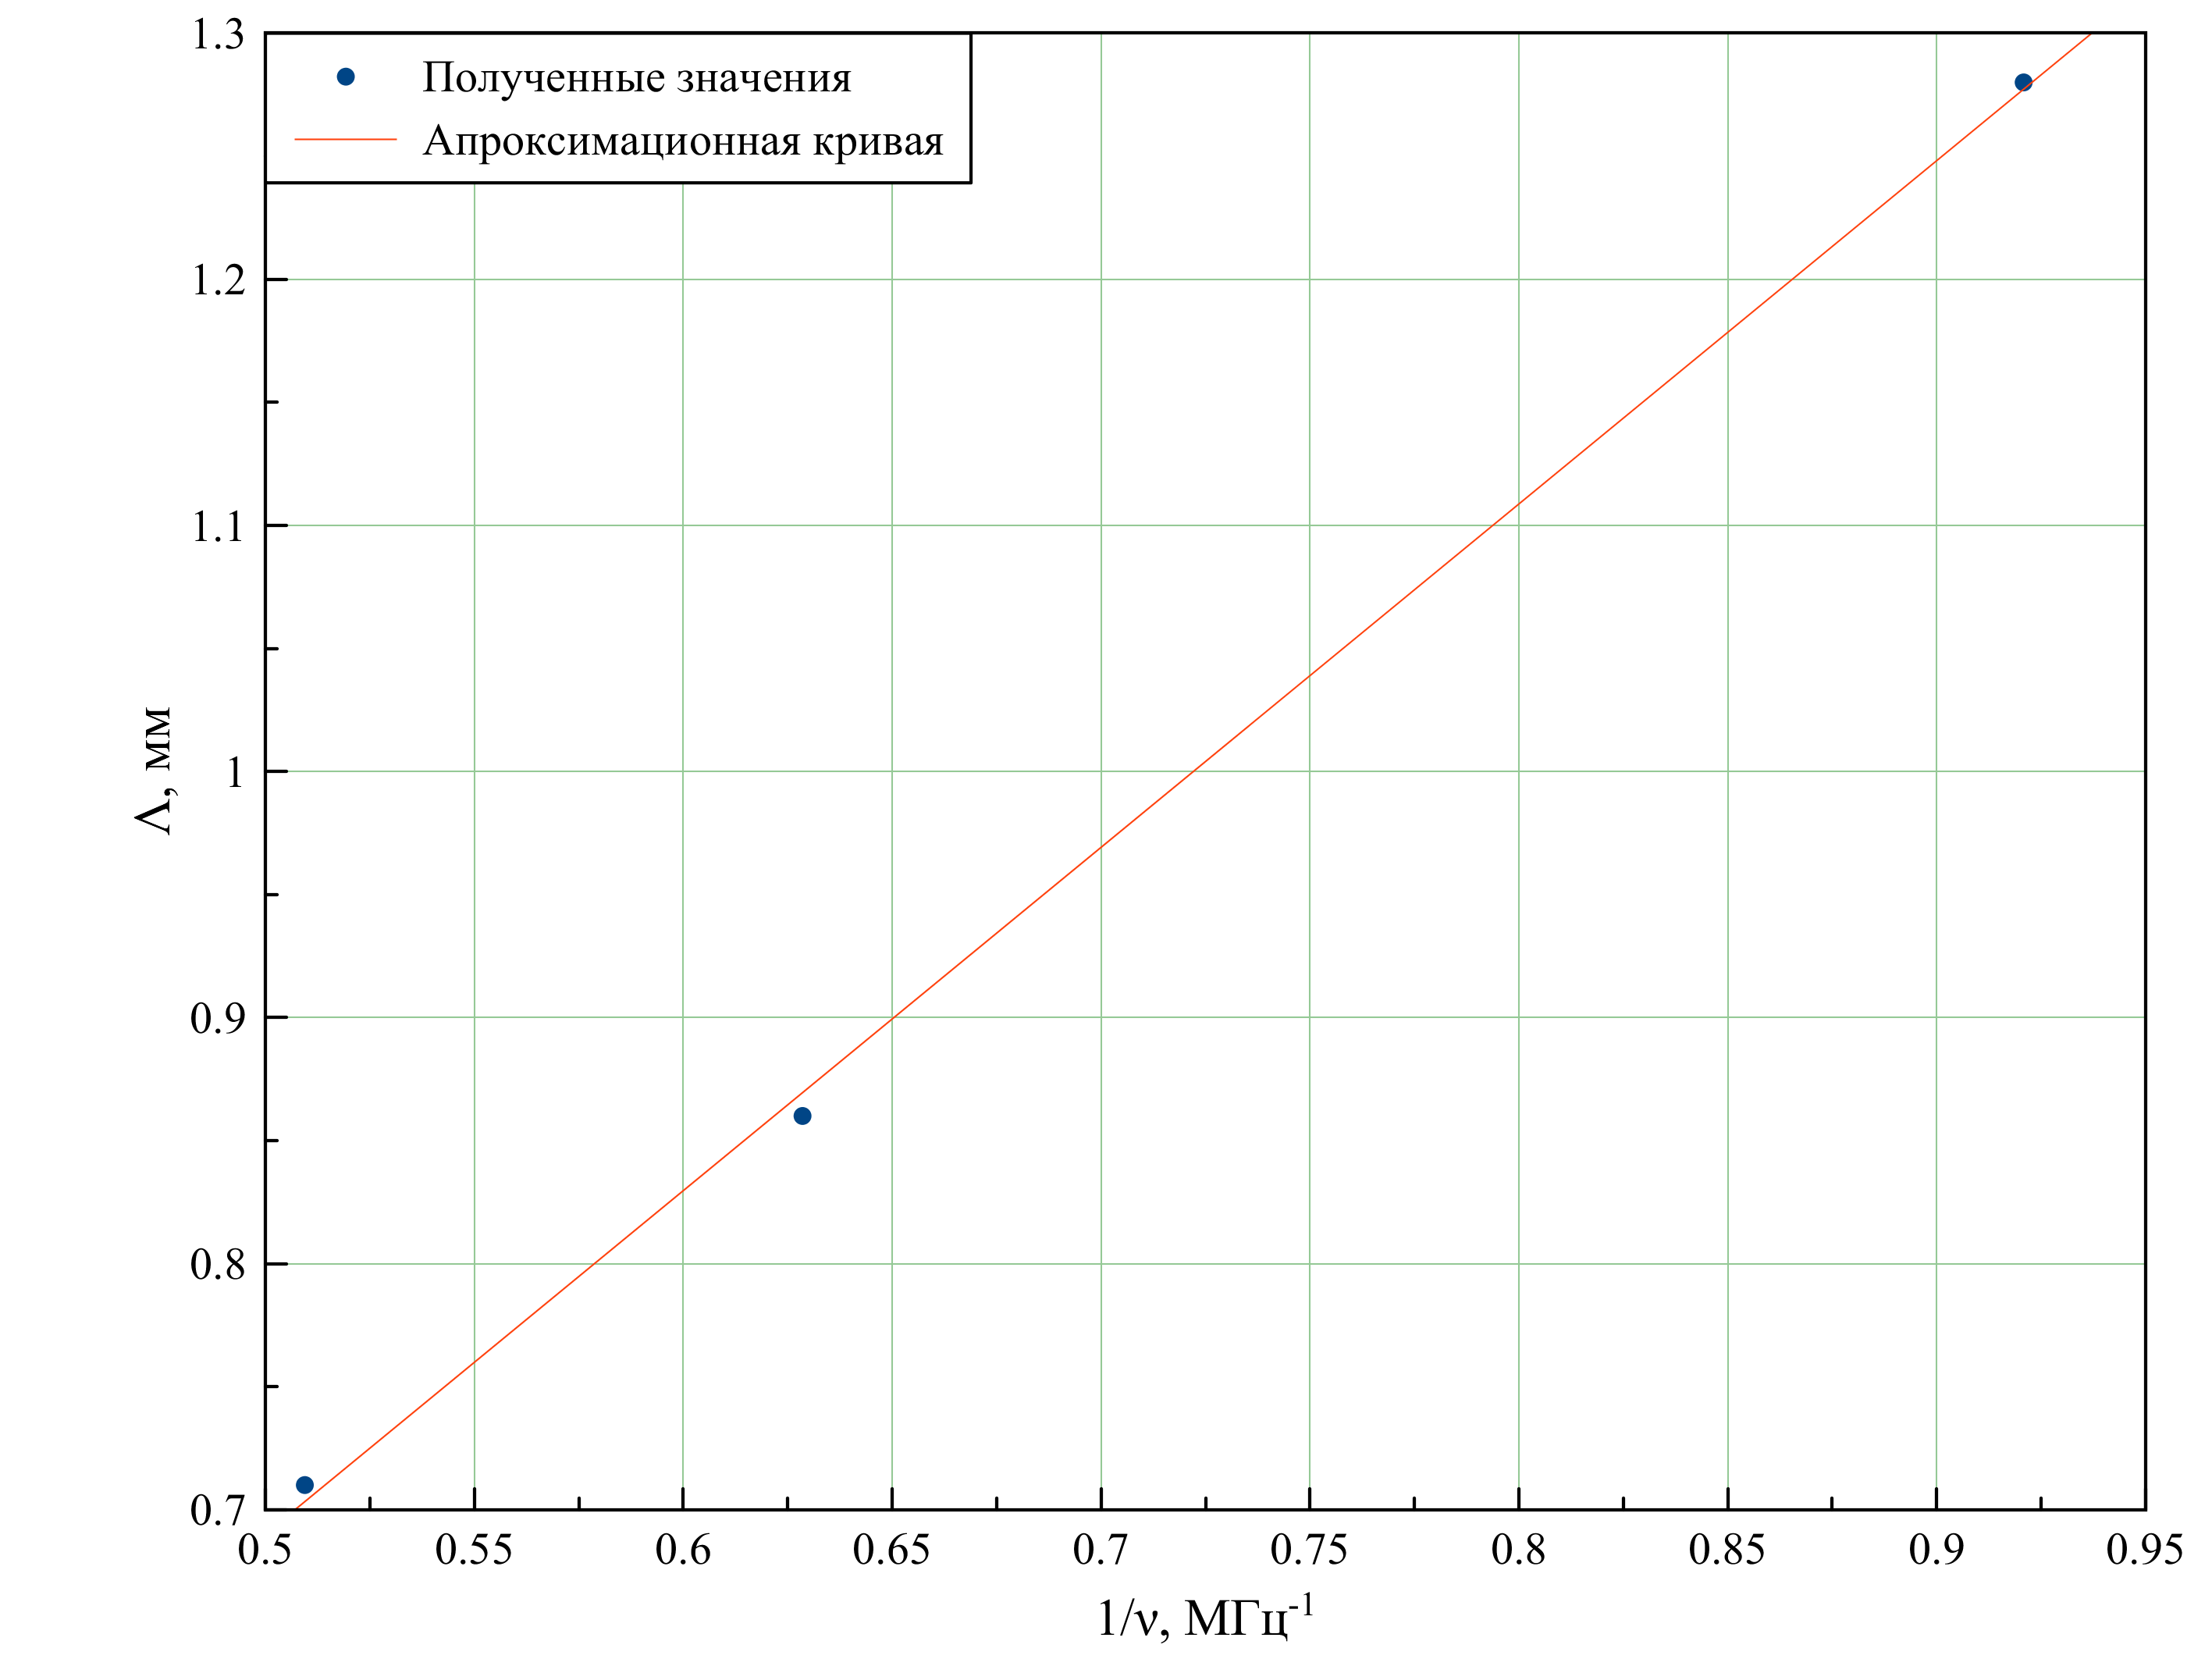
\includegraphics[width = 0.9 \textwidth]{graph3}
			\caption{График зависимости $\Lambda $ от $1/\nu$}
		\end{center}
	\end {figure}
	
\item По углу наклона графика найдем скорость звука в воде: 
$$\upsilon = \Lambda \nu = 1395\pm 4 \text{м/с}$$
\end {enumerate}

\section{Вывод}
Мы изучили дифракцию света на синусоидальной акустической решетке и пронаблюдали фазовую решетку методом темного поля.\\
Были получены следующие результаты:\\
$$\upsilon_\text{ар} = 1581 \pm 7\ \text{м/с}$$
$$\upsilon_\text{мтп} = 1395 \pm 5\ \text{м/с}$$
$$\upsilon_\text{табл} = 1500\ \text{м/с}$$




\end{document}